%% This is an example first chapter. You should put chapter/appendix that you
%% write into a separate file, and add a line \include{yourfilename} to
%% main.tex, where `yourfilename.tex' is the name of the chapter/appendix file.
%% You can process specific files by typing their names in at the 
%% \files=
%% prompt when you run the file main.tex through LaTeX.
\chapter{Codeable Objects}

\begin{center}
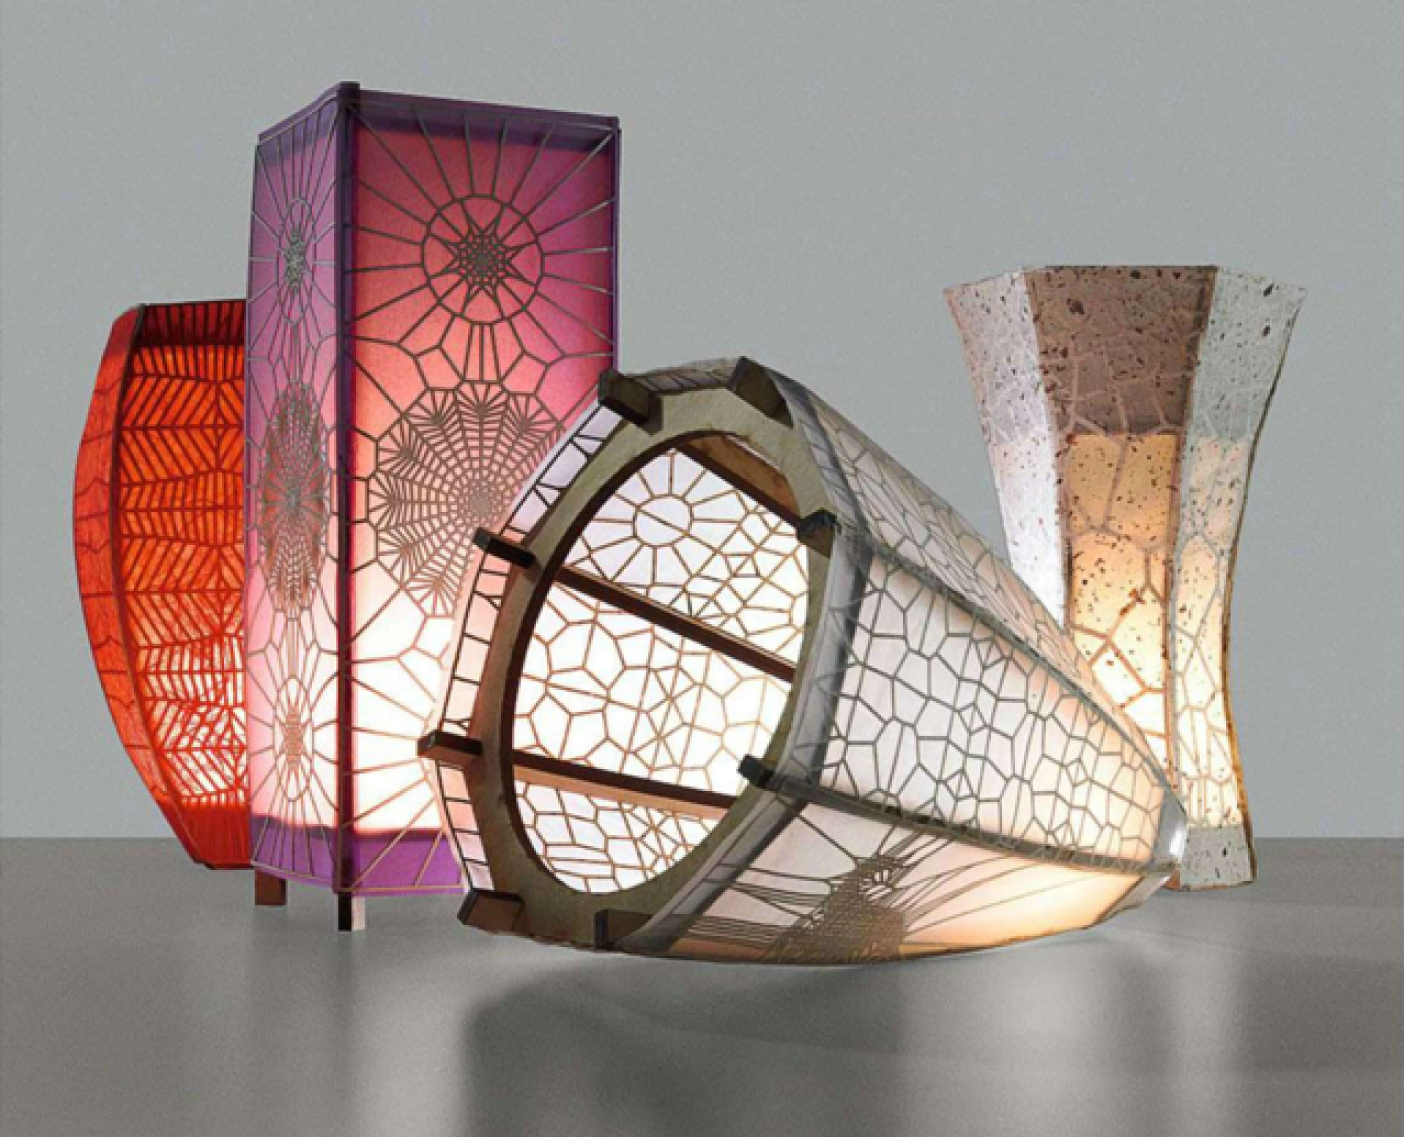
\includegraphics[width=\columnwidth]{images/finished_lamps.png}
\end{center}

Codeable Objects is computational design tool that allows people to design and export the toolpaths for a laser-cut lamp. Lamps possess an established function but can vary immensely in their form-factor. As a result, the domain of lamp design offers a wide set of design possibilities for a concrete and useful end product. By introducing lamp design in the context of algorithmic craft, my goal was to allow people to construct unique lamps comprised of computationally generated forms and patterns. 
\begin{center}
\begin{figure}[h!]
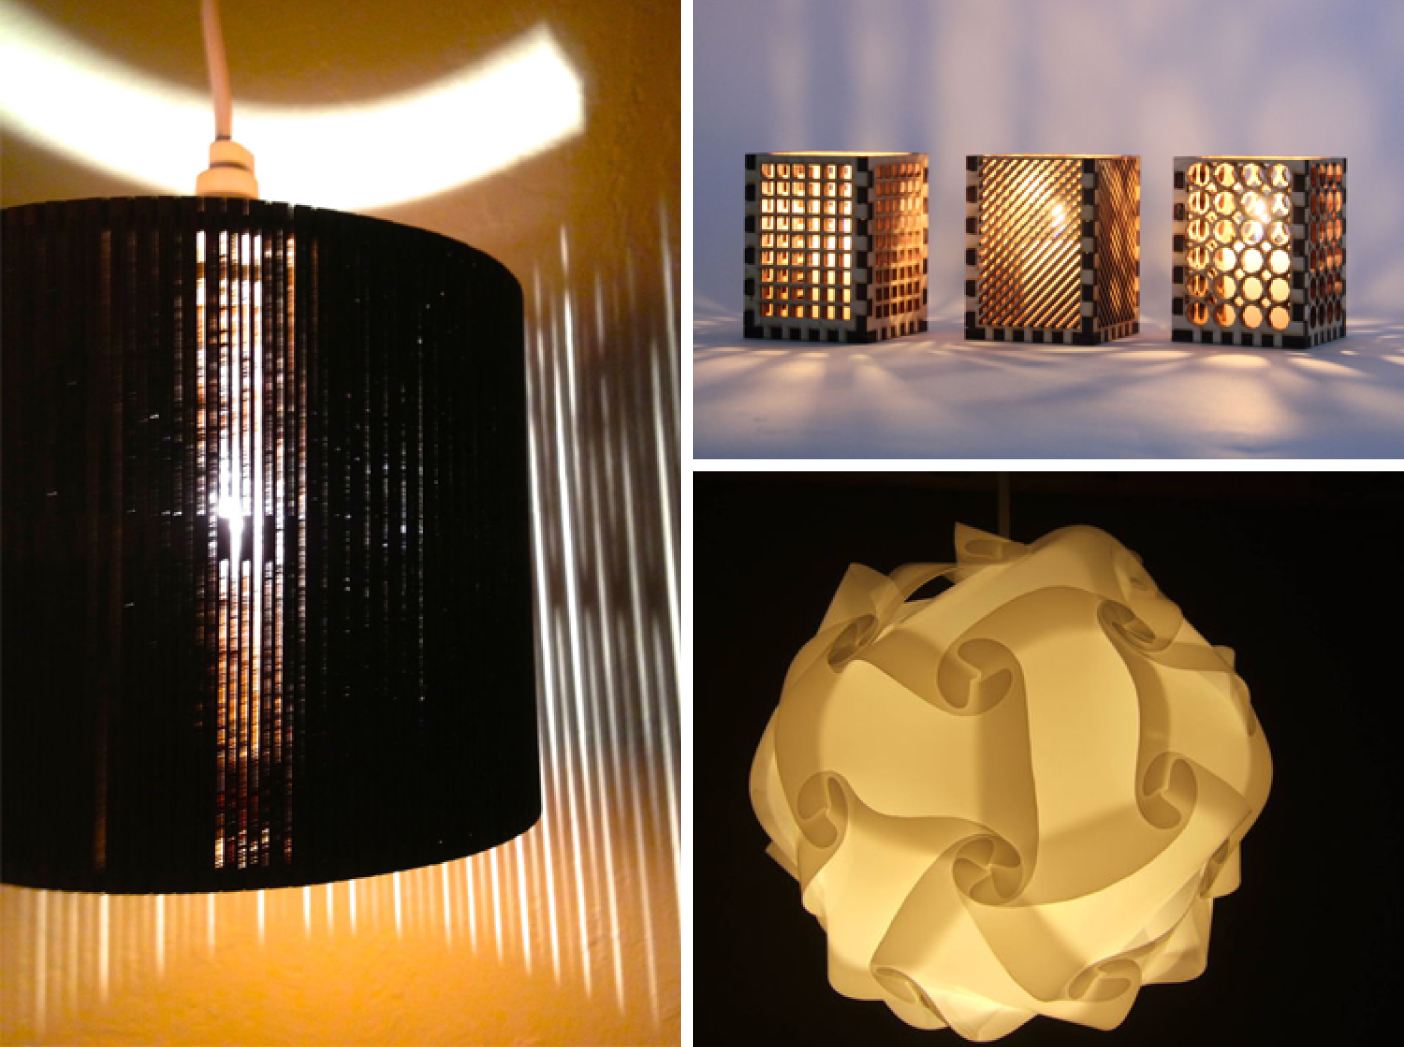
\includegraphics[width=\columnwidth]{images/instructables_lamps.png}
\caption{A selection of laser-cut lamps from Instructables}
\end{figure}
\end{center}
\section{Motivation}
There is a precedent for creating DIY lamps through digital fabrication. The Instructables community tutorial website has an entire section devoted to DIY lamps and many examples of patterns that use a laser cutter for fabrication. Many of these Instructables contain minimal design flexibility; they provide instructions that allow people to reproduce a lamp in the tutorial, but do not describe methods of deviating from the original design. The tutorials that do encourage design flexibility often require the person creating the lamp to use professional CAD tools to create their own design. In one popular laser-cut lamp Instructable, the author recommends using Solidworks to design the form and Illustrator to create the pattern on the shade \cite{instructables_lamp}. SolidWorks is more difficult to use than Illustrator, but has the benefit of being parametric. Conversely, Illustrator contains support generating aesthetic forms and patterns and is well suited to creating individual illustrations for laser cutting, but this program lacks the parametric functionality needed for the design of artifacts with multiple parts. Both tools are extremely challenging for first-time users.
\begin{center}
\begin{figure}[h!]
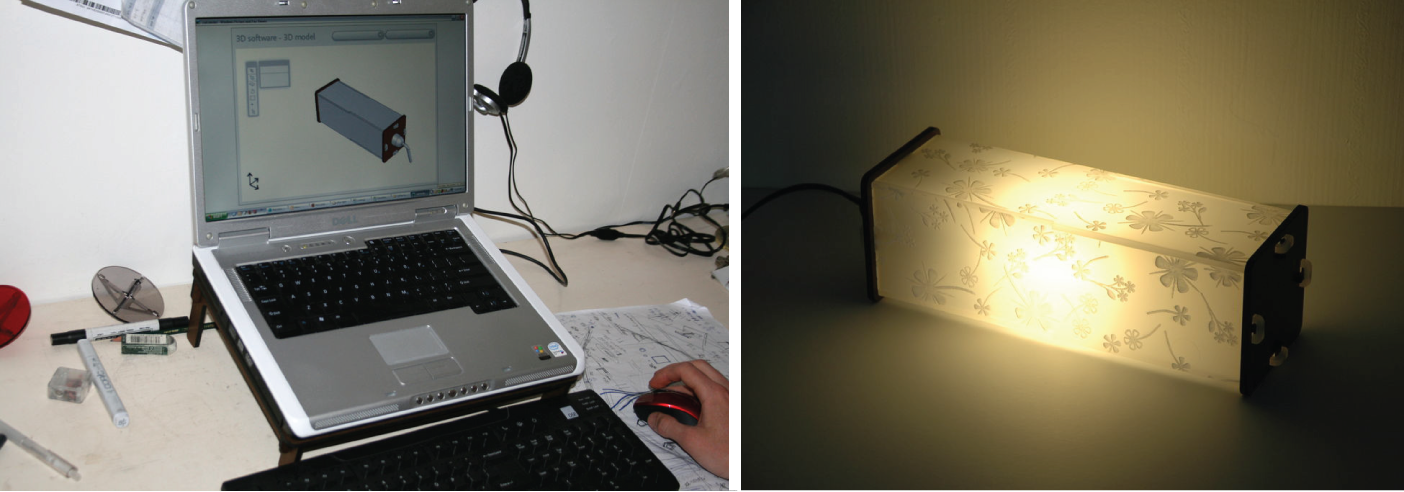
\includegraphics[width=\columnwidth]{images/solidworks_lamp.png}
\caption{Instructables lamp tutorial with SolidWorks design process}
\end{figure}
\end{center}
The use of existing software tools for lamp design presents other challenges. One common way to make laser-cut 3D forms is by assembling 2D press-fit pieces. I found that when creating 3D forms that were curved, it was extremely challenging in 2D CAD software to correctly size and design parts which would fit the faces of the lamp frame, creating the lamp shade. Although it is possible to create lamps from bare laser-cut frames, the shades themselves provided an excellent space for incorporating aesthetic illustrative elements. Without parametric functionality, however, it is difficult to modify the aesthetics and form of the lamp in a back-and-forth manner. Computational design offers a solution to many of these problems, while simultaneously providing a form of constructive engagement in programming, fabrication, and craft.

\section{Tool Description}
The first version of Codeable Objects attempted to combine parametric manipulation, aesthetic pattern generation, and the conversion of a 3D form to 2D parts into a single computational tool for lamp design. The lamp itself was comprised of five basic parts, a wooden press fit frame, a set of vellum pieces that fit over the frame to act as a shade, a set of cardstock pieces with a pattern that fit over the shades, and a pre-made standard light fixture that fit into the frame (figure:\ref{fig:lamp_parts}.)
\begin{center}
\begin{figure}[h!]
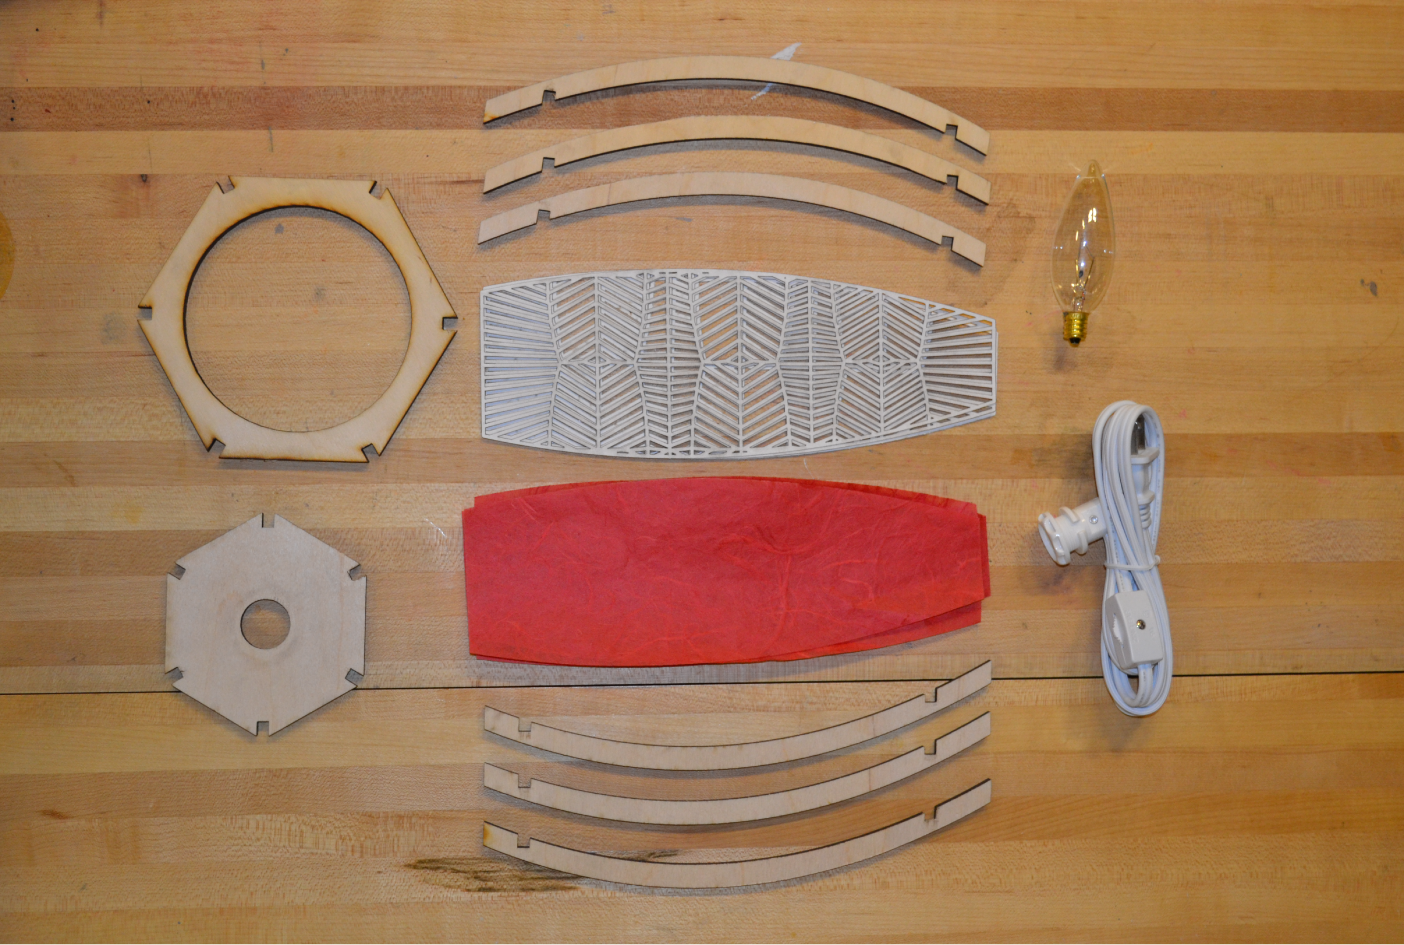
\includegraphics[width=\columnwidth]{images/parts.png}
\caption{The individual parts of a lamp}
\label{fig:lamp_parts}
\end{figure}
\end{center}
\vspace{-20pt}

Codeable Objects was developed as a programming library for Processing and contained a set of programming methods that allows the user to describe the lamp, and define the tool paths for all three materials. In the first version of the library, all design took place via textual programming and keyboard commands. There are four main functions in the Codeable that determine the height, top width, middle width, and bottom width of the lamp. The library also provided access to an additional set of methods that control the number of sides, the resolution of the curve, and the position of the internal structural supports. To facilitate the construction process, notches are automatically generated in all of the parts to allow the lamp to be press-fit together. The shades are also automatically generated to fit the form specified by the user. The inclusion of this feature gives the user freedom to customize the shape of the lamp without having to worry about the mechanics of construction.

\begin{center}
\begin{figure}[h!]
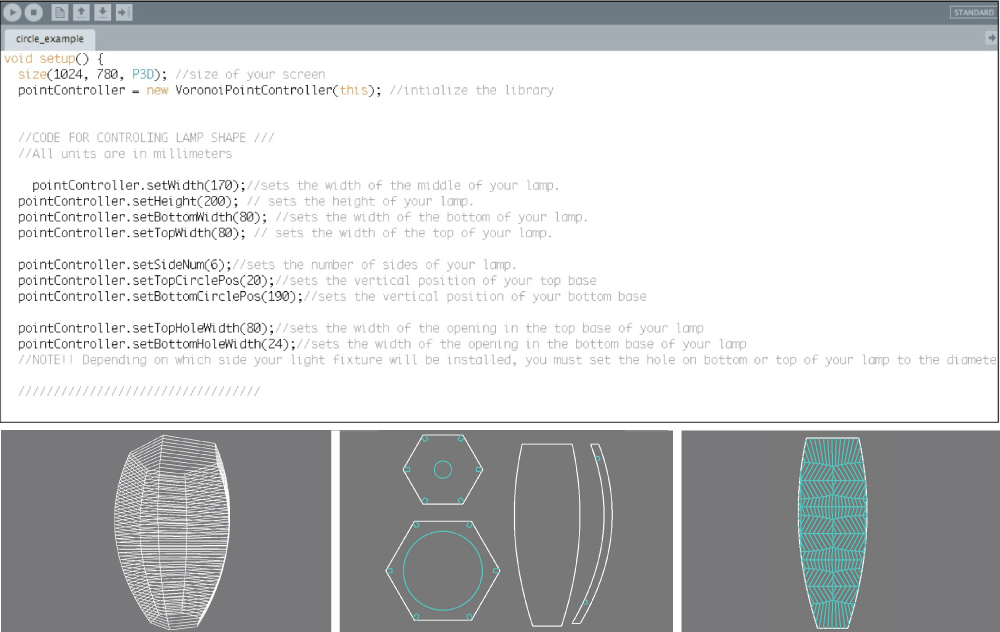
\includegraphics[width=\columnwidth]{images/codeable_objects_v1.jpg}
\caption{The first version of Codeable Objects, with only text-based interaction}
\label{fig:codeable_objects_v1}
\end{figure}
\end{center}
\vspace{-20pt}

Codeable Objects also includes a second set of programming methods that allows users to describe the decorative components of the lamp by specifying coordinates in polar or cartesian space. When compiled, the coordinates are used by the application to calculate a design using a Voronoi diagram, which is automatically clipped to the dimensions of the lamp shade. As the form of the lamp is altered, the shades and patterns are adjusted to fit. Once the code is compiled, a graphic preview is displayed. For the pilot version, users could use key-commands to toggle between a view of the form of the 3D form of lamp, the Voronoi-diagram pattern, and a 2D preview of the press-fit parts (fig:\ref{fig:codeable_objects_v1}.) A final key-command allowed for the resultant design files to be exported as three separate PDFs containing the paths for the press-fit frame, the shades, and the pattern files. The functionality of Codeable Objects was designed to provide a platform that allowed for flexible computational design and the creation of complex forms and patterns, while greatly simplifying the process of translating the design to a suitable format for digital fabrication. The laser cutting-process produced parts that expedited the construction process, but still but required care and dedication in assembly. Combined, these properties were designed to foster an experience that merged programming, digital fabrication, and hand-craft, and which hopefully resulted in a useful finished artifact.
		
\section{Evaluation}
The first evaluation of Codeable Objects was conducted  during a six-hour workshop with a group of nine graduate students ranging in age from 24-34. Five participants were women. According to self-reported pre-survey data, all but one of the participants was an intermediate- to-experienced programmer. Five of the nine had previous experience with Processing. The participants indicated they had little or no prior experience in design. What experience they had was primarily gained in high school art classes and college elective courses. During the workshop, each participant engaged in the design and fabrication of a lamp. Participants received instruction in the use of Codeable Objects and a basic explanation of the principles behind the geometry of the lamp. The pilot version of Codeable Objects was packaged with a set of example programs that contained the basic code for initializing the library and defining the parameters of the lamp, along with a variety of point generation methods. The examples included algorithms to generate spirals, circles, and grids in points. Participants also were provided with access to construction materials, and received training in the use of the laser cutter. They were given approximately four hours to design the structure and ornamentation of a lamp, followed by two hours for fabrication and assembly.

\begin{center}
\begin{figure}[h!]
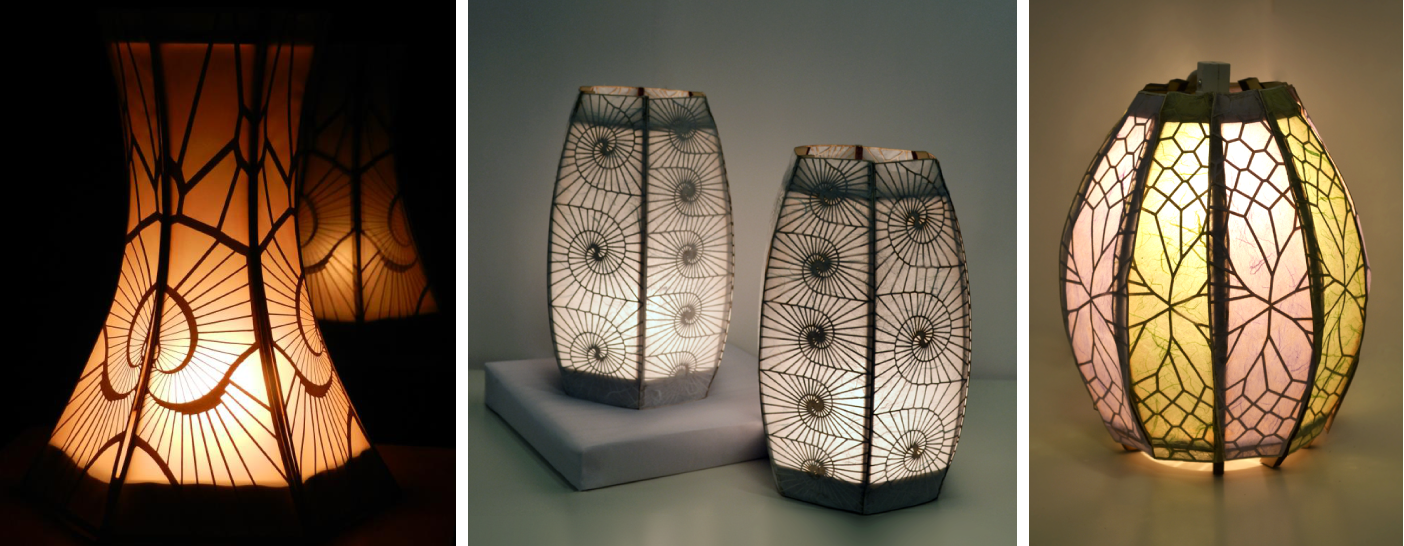
\includegraphics[width=\columnwidth]{images/finished_lamps2.png}
\caption{Several of the finished lamps from the first workshop}
\label{fig:finished_lamps}
\end{figure}
\end{center}
\vspace{-20pt}

\section{Results}
All but one of the participants in the lamp workshop successfully completed a lamp. The one exception was a user who wished to incorporate a specialized light fixture into her piece, but unfortunately, she damaged her parts while waiting for the fixture to arrive. The participants with little or no prior programming experience primarily relied upon tweaking or remixing the example programs to design the form and pattern of their lamp. Those with more programming experience experimented with the library to produce a wide range of forms and patterns. One participant wrote a program that decomposed a black-and-white image into a point cloud and used that as the basis for her pattern. Another participant wrote a program that used a Gaussian distribution of points to achieve the gradual variation he desired in his final pattern. 

 The assembly of parts required additional time beyond the duration of the workshop for most participants. This was partially the result of the bottleneck in using the laser cutter; one fabrication machine split among many participants resulted in long wait times. The craft and construction components of the project took longer than expected as well. All of the participants returned after the workshop to complete their projects. Some participants chose to add additional steps to the construction process, such as sanding their parts. The physical objects produced were both attractive and functional and participants displayed their lamps in their offices and homes after completion. One participant returned several days later to build a second lamp so that he had a matching set for his bedside tables (figure:\ref{fig:finished_lamps}.)		
		
		
\section{Discussion}

Because of their prior expertise, the experiences of the majority of the participants in the first study are not indicative of the feasibility of Codeable Objects for novice programmers. Their experiences instead stand in contrast to the experience of the novice coders in the successive workshops and provide important information about the usability and workflow of the software. Some of the experienced programmers provided immediate practical assistance by developing new example programs for Codeable Objects, including an extremely popular program the creation of cosine and sine wave patterns. Because the library was open-source, participants were able to submit upgrades to the interface design and functionality during the workshop itself, which later were incorporated into the core version.

The experienced programmers in the lamp workshop exhibited limited knowledge of computational design prior to the start of the workshop. When asked in the pre-workshop surveys how they thought programming, design, and craft could be combined, people were either uncertain, or described the combination as method to create dynamic interactivity, rather than a tool for the design of form and pattern:
\begin{quotation}
\textit{``You can combine software and hardware and make craft more dynamic (e.g. sensors)."}
 \\Lamp Participant 1
\end{quotation}
\begin{quotation}
\textit{``[programming] gives [you] the ability to make something dynamic."}
 \\Lamp Participant 3
\end{quotation}

Following the workshop, participants demonstrated an awareness of some of the specific affordances of computational design and the benefits of combining computational design with digital fabrication:
\begin{quotation}
\textit{``I understand now how programming can be used for quick prototyping and mockups that can be used to inform final design decisions. This is easy [and] helpful when using physical materials where mistakes can be costly."}
\\Lamp participant  2
\end{quotation}

\begin{quotation}
\textit{``Using programming in the design process adds some exciting and unique capabilities over traditional design and crafting, including mixing in different algorithm and ideas from other existing software, and rapid prototyping of complex designs."}
\\Lamp participant 6
\end{quotation} 

Participants were also pleased with the creative affordances of the tool and described how the software enabled them to expand their programming abilities to the realm of art and craft with greater success: 
\begin{quotation}
\textit{``I think programming makes designing more accessible because you don't have to be able to draw or paint."}
\\Lamp participant 4
\end{quotation}

\begin{quotation}
\textit{``I love the idea of being able to combine my interest in programming for creative expressions."}
\\Lamp participant 6
\end{quotation}

One participant remarked that she had always believed that she was terrible at art and making the lamp had altered that perception. Although the primary objective behind Codeable Objects was to make a form of algorithmic craft that was accessible to non-programmers, in the first workshop, it provided a pathway for programmers to apply their skills to design and craft. From these responses, it is apparent that even among experienced programmers, algorithmic craft has the potential to expand people's understanding of the applications of programming and motivate them to apply computation to other forms of production and expression.

Several participants also put forth detailed critiques of the programming process, which brought up other questions about the practice of computational design. One participant reacted against defining the generative qualities of the Voronoi diagram patterns as a design method:
\begin{quotation}
 \textit{``Changing the parameters didn't always generate the pattern you have in mind. It was more like generating a few semi-random patterns, and you choose one that looks good. It is rather a trying-and-choosing rather than designing /making something you planned to have. I think "design" involves "intention" and "planning." Programming, crafting, and design should be combined in the way that entails prior planning and intentions as opposed to cutting together the semi-random choices, which could be good but I wouldn't call that design."}
 \\Lamp participant 6
 \end{quotation}
 
As this quote indicates, the attributes of randomness and generativity do not automatically lead to optimal or good design decisions. Some deciding factor has to play a role in the process, but the criteria for this decision are often ambiguous. This criticism touches on a core debate about the role of conscious design and the restriction of intuitive creativity in computational practices. The emergence of comments like this are encouraging because they reflect the engagement of the participants in a critical evaluation of the creative implications of this form of creation. 

\subsection{Challenges}
There were elements of the process that were problematic for the participants. It became clear during the workshop that textual programming was not the best method to design the form of the lamp. Many of the participants became frustrated about having to set the parameters and then wait for the compilation process to complete before they could view the results. This issue was addressed partly in subsequent versions of the tool by replacing the textual parameters with a set of sliders in the compiled application, which would adjust the form in real time across each of the views (figure: \ref{fig:slider_interface}.)
\begin{center}
\begin{figure}[h!]
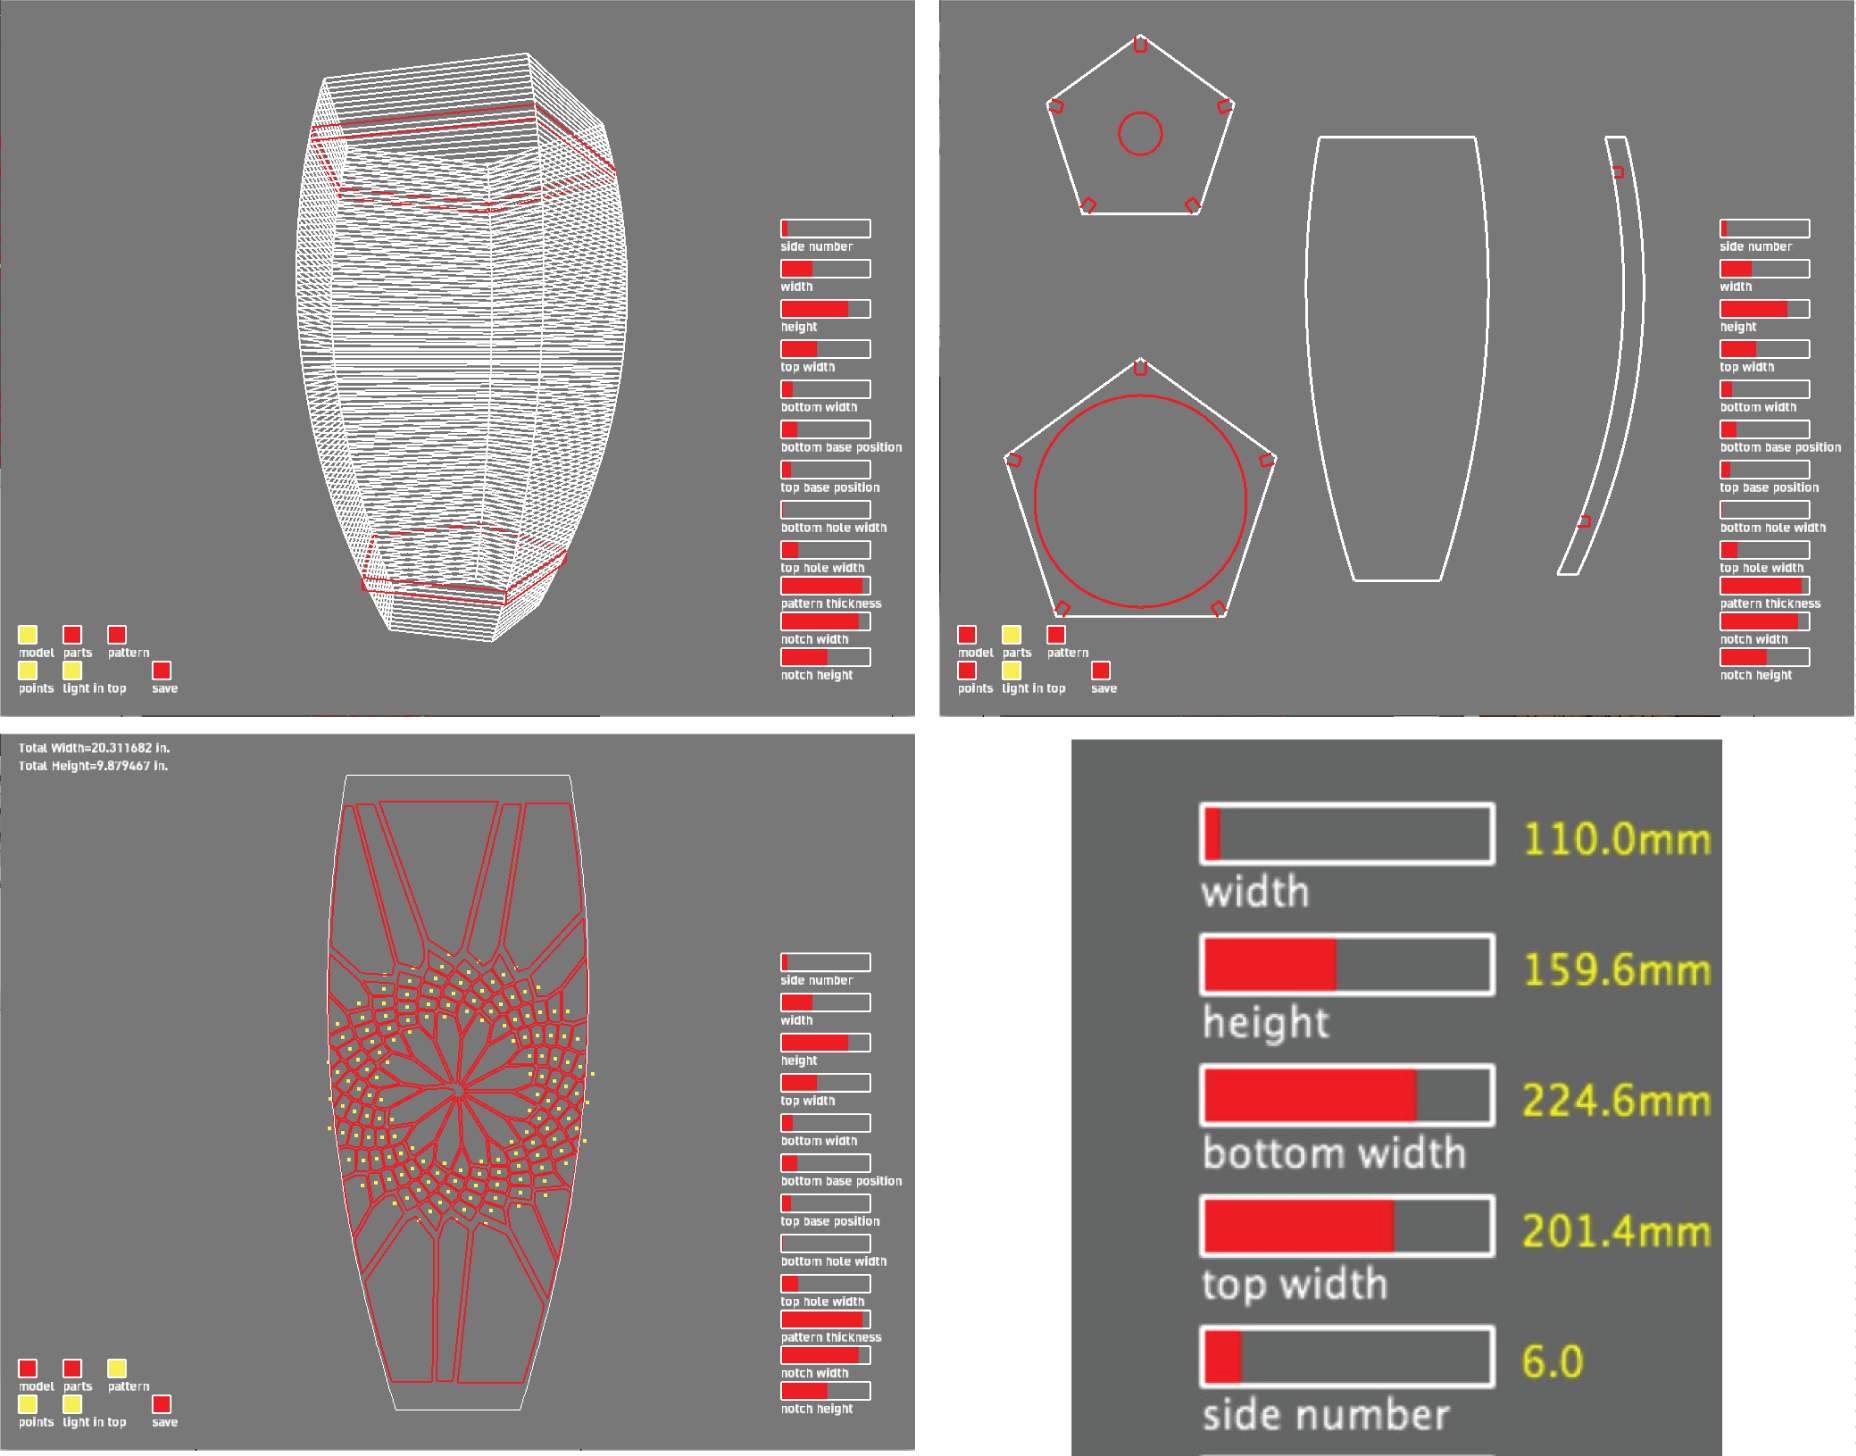
\includegraphics[width=\columnwidth]{images/slider_interface.png}
\caption{Revised graphic view with sliders}
\label{fig:slider_interface}
\end{figure}
\end{center}

The textual programming method was useful for creating pattern on the shades. The simple method of specifying points in a programming context provided a space for creativity and resulted in greater variation in the lamps. If the tool had relied on a more standard set of GUI components, like sliders to control the point generation, it is doubtful that the same range could have been achieved. On the other hand, it was clear that the less -experienced programmers had difficulty independently designing the patterns of their lamps, and relied primarily on adjusting and remixing existing examples. 

Another restriction of Codeable Objects was apparent in the design process. Although adjusting the parameters and input values to a system can be considered a form of design, it only touches the surface of the design opportunities made possible with algorithmic craft. With Codeable Objects, people cannot modify the program to define the range of forms and patterns that are possible unless they alter the source code of the library. This limitation prevented the evaluation of some of the more interesting computational design processes such as allowing people to create personal stylistic abstractions for patterns and forms by writing their own algorithms. The stylistic limitations of Codeable Objects contributed to the high rate of success in project completion, and the general attractiveness of the resulting projects, but they also constrained the design flexibility. 

One other defining component of the Codeable Objects pilot workshop was the contrast between the difficulties that arose through computational design and digital fabrication and the challenges in crafting. The difficulties people experienced while designing and fabricating their projects were often discrete; such as correcting for mathematical error in coordinate placement, or having the incorrect setting on the laser cutter. More complex problems arose in these contexts as well, such as confusion on the algorithms for placing points, however they were often problems that could be addressed through verbal instruction and explanation. The challenges encountered in the crafting session were of a material or physical quality. People struggled with finding the best techniques for assembling the parts and finishing individual pieces so that the product maintained an attractive appearance. Most participants were surprised at the amount of time required to complete the physical assembly and were sometimes frustrated when variations in the crafting process violated the precision and perfection of the digital design and laser-cut parts. 

Some of the frustrations in the physical construction process were addressed in subsequent workshops by creating a paper variation of the lamp that was faster and easier to assemble and required no gluing (figure: \ref{fig:paper_lamp}.) In addition, a feature was added to the software which reported the approximate material size required for a design, so that users could ensure theirs would fit on the bed of the laser cutter. 
\begin{center}
\begin{figure}[h!]
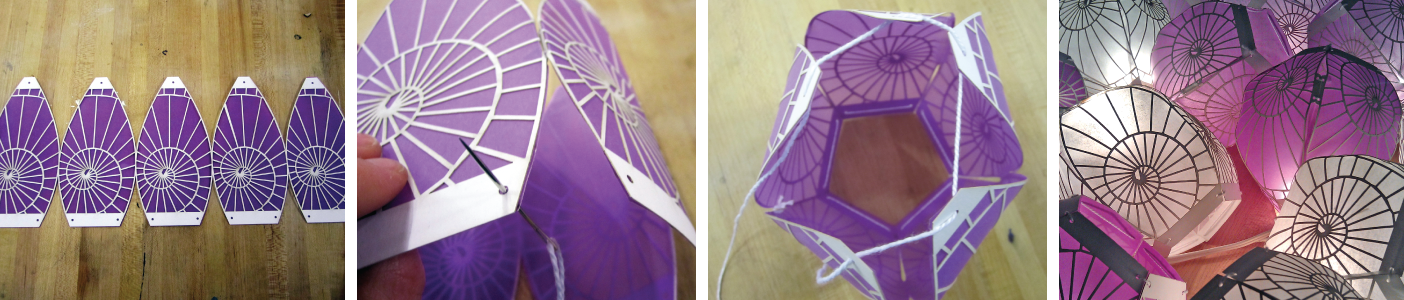
\includegraphics[width=\columnwidth]{images/paper_lamps.png}
\caption{The revised paper lamps}
\label{fig:paper_lamp}
\end{figure}
\end{center}

Frequently, a user's experience can be improved with changes in the interface and artifact design, In thinking about how to approach improvements, it is useful to distinguish between frustrations that are the result of a software interface and learning processes that are inherent in design and craft. In both craft and computation, care and practice contribute to improved results. Furthermore in craft, material variation and inconsistency can be difficult to manage, but these factors also can contribute to the uniqueness and value of an object. The process of supporting people in algorithmic craft is not just about building tools that make the programming process easier and the crafting component less prone to risk. Instead, computational tools should be designed to remove technical barriers in programming and fabrication so that people can address the more interesting (and often more difficult) design challenges of envisioning and refining computational systems. Craft processes should be feasible to achieve, but also recognize that part of the pleasure and accomplishment of crafting comes from the risk and difficulty it entails. 

\section{Summary}
Codeable Objects allowed people to produce useful and beautiful objects with personal value through a relatively pleasurable experience in computational design, digital fabrication and craft. It also produced in experienced programmers a recognition of the aesthetic and design potential of computation, and stimulated questions about the role of conscious choice in computational design. The workshop demonstrated the importance of immediate visual feedback for informing design decisions, and it indicated the importance of applying textual programming to formats that clearly demonstrated its advantages. The workshop highlighted the utility of open-sourcing algorithmic crafting tools. Making the source code of Codeable Objects available to the advanced programmers in the workshop lead to immediate innovations in the functionality of the software. For subsequent tools, my goal was to build on these success while attempting to diminish some of the design limitations of Codeable Objects. I also began working with a representative group of young designers with limited programming experience. 